\documentclass{article}
\usepackage{tikz}

\begin{document}

\begin{figure}[h]
    \centering
    \begin{tabular}{cc}
        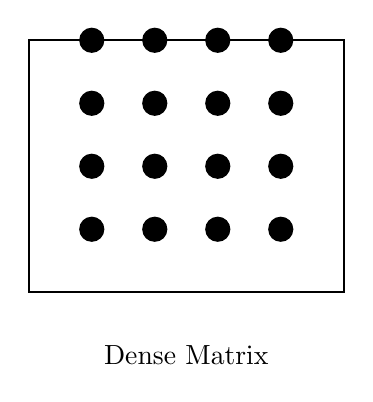
\begin{tikzpicture}[scale=0.8]
            \draw[thick] (0,4) -- (5,4) -- (5,0) -- (0,0) -- cycle;
            \foreach \x in {1,...,4} {
                \foreach \y in {1,...,4} {
                    \fill (\x,\y) circle (0.2);
                }
            }
            \node at (2.5,-1) {Dense Matrix};
        \end{tikzpicture}
        &
        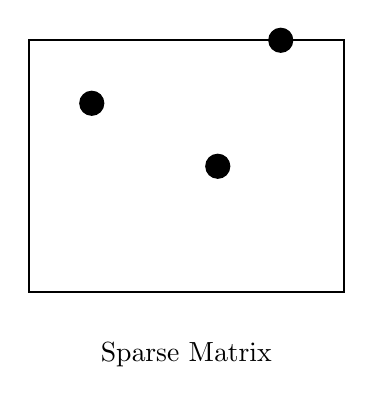
\begin{tikzpicture}[scale=0.8]
            \draw[thick] (0,4) -- (5,4) -- (5,0) -- (0,0) -- cycle;
            \fill (1,3) circle (0.2);
            \fill (3,2) circle (0.2);
            \fill (4,4) circle (0.2);
            \node at (2.5,-1) {Sparse Matrix};
        \end{tikzpicture}
    \end{tabular}
    \caption{Comparison of Dense and Sparse Matrices}
    \label{fig:dense_sparse_matrices}
\end{figure}

\end{document}